% 2-3 page summary of the findings of the Backgrounds WG
\label{app:background}
% editors: Juliette Alimena, Martino Borsato, Sascha Mehlhase
% largely based on https://goo.gl/fw95iR

% -----------------------------------------------------------------------------------
\section{Introduction} % Sascha, all
% -----------------------------------------------------------------------------------

For many searches for long-lived particles, the (main) background is not stemming from SM processes, but arises from \textit{external sources} or is even instrumental and/or of algorithmic nature. This section gives an overview on common \textit{non-physics} background and means to estimate or control these types of background.

% -----------------------------------------------------------------------------------
\section{Known long-lived particles} % Martino
% -----------------------------------------------------------------------------------
Weak decays of SM particles normally have displaced vertices at the boosts typically encountered the LHC. The searches for signature at low enough LLP mass and lifetime suffer from large backgrounds due to displaced SM decays. One simple example is found in the search for long-lived dark photons~\cite{Aaij:2017rft} decaying to $\mu^+ \mu^-$, which drastically looses sensitivity when getting too close to the $K_{\rm S}\rightarrow\pi^+\pi^-$ invariant mass despite the very low $\pi\rightarrow\mu$ mis-ID.

Decays of b-hadrons give displacements of few millimetres and can be indistinguishable from a LLP with mass few tents of GeV decaying to a pair of jets. Requiring a large track multiplicity of the displaced vertex and performing a mass fit to the dijet invariant mass can help to significantly reduce the effect of this background (see for example~\cite{CMS:2014wda, Aaij:2017mic}.
Backgrounds from heavy flavours are typically more abundant in the forward region (e.g. if the signature searched is a LLP from a SM Higgs decay). However, the LHCb forward detector, being designed to study these SM decays, typically is also capable of rejecting them more effectively.

% -----------------------------------------------------------------------------------
\section{Real particles generated in the detector} % Martino
% -----------------------------------------------------------------------------------

% -----------------------------------------------------------------------------------
%\subsection{Nuclear interactions} % I think maps for nuclear interactions are the same that are used for for photon interactions.
% -----------------------------------------------------------------------------------
Interactions of particles produced in the $pp$ collision with nuclei of the detector material can give displaced vertices and fake a LLP signal. Vertices from these interactions will be positioned in the detector material volume and are therefore effectively vetoed by using detailed material maps. 

LHC detectors have developed tools internal to the collaborations to define a material volume to be vetoed. Maps from ATLAS and CMS obtained with data collected in 2010 can be found in ~\cite{Aaboud:2016poq} and \cite{CMS:2010nua} and are valid for the Run 1 configuration. More recent maps, for the Run 2 detectors configurations can be found in ~\cite{Aaboud:2017iio} (see also Figure~\ref{fig:materialmaps}) and \cite{CMSmaterial} for ATLAS and CMS, respectively.

\begin{figure}[h]
  \centering
  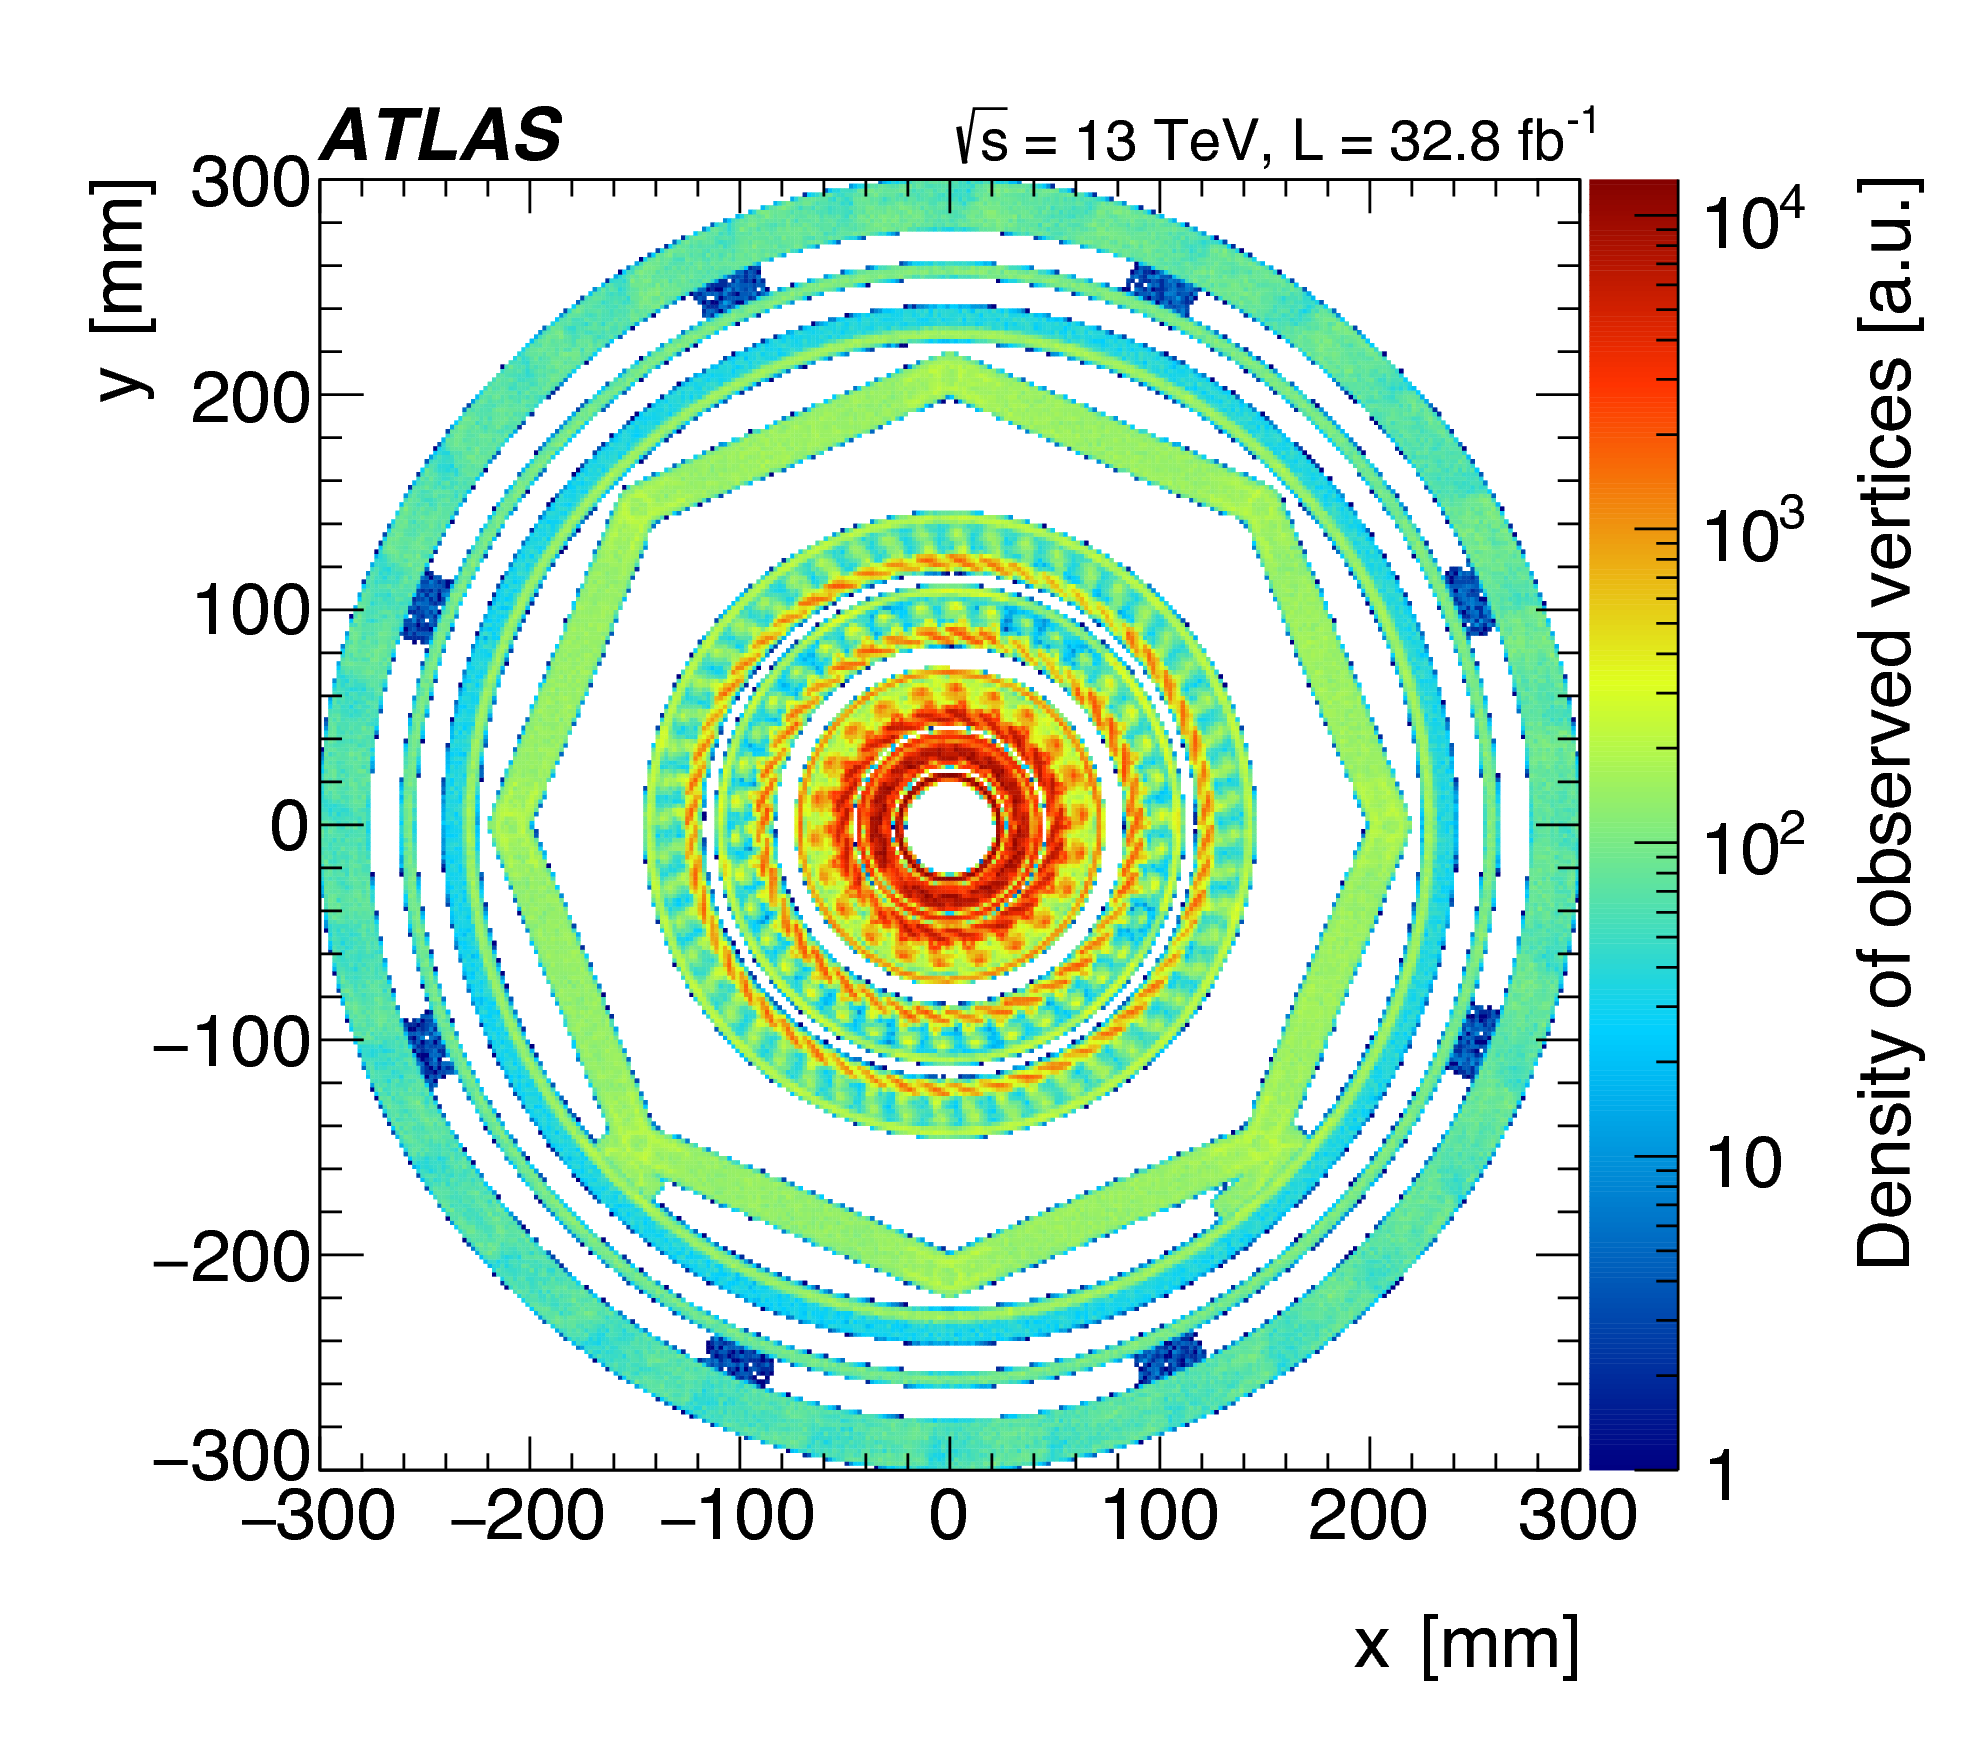
\includegraphics[width=0.7\textwidth]{figures/atlasmaterial.png}
%   \hfill
%   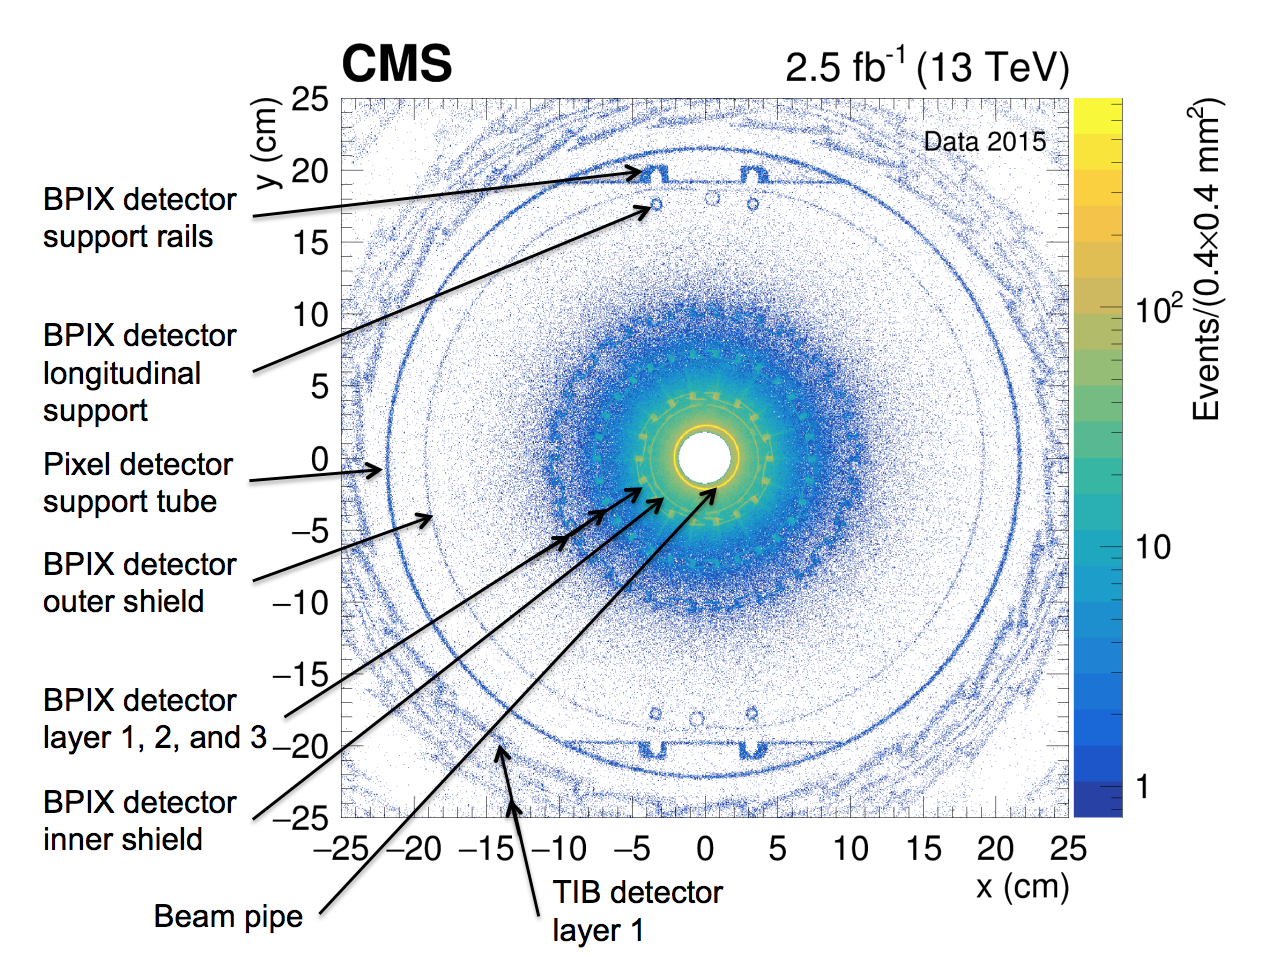
\includegraphics[width=0.48\textwidth]{figures/cmsmaterial.png}
  \caption{Examples of material maps for ATLAS~\cite{Aaboud:2017iio}
  % and CMS~\cite{CMSmaterial}}
  }
  \label{fig:materialmaps}
\end{figure}

LHCb recently developed a precise material map of the Vertex Locator (VELL) using beam-gas collisions. This type of collisions is mostly free from long-lived heavy flavour background and allows to cover precisely the whole VELO geometry, not only the region close to the interaction point. This map was used to veto photon conversions to dimuons, which is the main background affecting displaced dark photon searches at low mass~\cite{Aaij:2017rft}. As a rule of thumb, LHCb material interaction background is dominant for vertices at a distance from the beam axis larger than 6 mm (where the VELO material begins). Below 6 mm the background is dominated by heavy flavour decays~\cite{Ilten:2016tkc}.

The LLP community is interested in using public tools for material maps of LHC experiments to improve the reliability of sensitivity studies to signatures with displaced vertices. The availability of such tools in fast parametric simulations such as Delphes~\cite{deFavereau:2013fsa} could be very interesting.

%ATLAS 7 TeV \cite{Aaboud:2016poq} (QUESTION: is it valid for Run 2?)
%CMS 7 TeV \cite{CMS:2010nua} 
%CMS 13 TeV \cite{CMS-DP-2016-073,CMSmaterial} (there is no paper, am I right?) JA: We have a public detector performance note (CMS-DP-2016-073) and a newer public twiki than the original one you cited (I updated the reference). The the paper is about to enter CWR, so not public yet. 

% -----------------------------------------------------------------------------------
\section{Real particles generated outside the detector} % Juliette
% -----------------------------------------------------------------------------------

There are several types of real particles generated outside the detector that could be sources of background in a LLP search. 

% -----------------------------------------------------------------------------------
\subsection{Cosmic muons} % Juliette
% -----------------------------------------------------------------------------------

For example, cosmic rays from the atmosphere could enter the detector as cosmic-ray muons. These cosmic-ray muons could be reconstructed as displaced muons in the muon system or as displaced jets in the calorimeters. If cosmic-ray muons are reconstructed in the muon systems, they will typically appear as two back-to-back muons with $\phi$ values near $\pm\pi/2$. The rate of cosmic muons in the detector is about 500~Hz at L1, but depending on the HLT path and the offline selection used, the rate of cosmic-ray muons entering a given LLP analysis is generally much less.

Cosmic-ray muons are typically an important background source to consider for displaced signatures, especially those with large displacements~\cite{Khachatryan:2015jha, Chatrchyan:2012dxa, Khachatryan:2010uf, Aad:2012zn,Aad:2013gva}. Cosmic-ray muons are generally only an issue for CMS and ATLAS analyses, but not for LHCb analyses, since LHCb has only forward coverage. 

For many analyses, cosmic-ray muons can be rejected with a simple veto on back-to-back dimuons. However, in some analyses, this veto is not optimal for the signal acceptance or it is insufficient. Another often-used way to minimize the contribution from cosmic-ray muons is requiring high-momentum muons and/or high-energy jets, since cosmic-ray muons have a falling $p_{T}$ spectrum. In addition, if a search primarily looks for inner-tracker or calorimeter objects, cosmic-ray-muon events can be rejected by requiring little muon system activity~\cite{Khachatryan:2015jha, Chatrchyan:2012dxa, Khachatryan:2010uf}.

If the cosmic-ray muon background is significant for an analysis, it can be estimated using data from dedicated cosmic data-taking runs or from empty bunches in $pp$ collision runs~\cite{Khachatryan:2015jha, Chatrchyan:2012dxa, Khachatryan:2010uf}. Cosmic-ray-muon simulations can be made, but in many LLP analyses, a data-driven approach is favoured. Timing information in the calorimeters or the muon systems can be used to discriminate the signal from  cosmic-ray muons, sometimes in conjunction with impact parameter variables.

% -----------------------------------------------------------------------------------
\subsection{Beam halo} % Juliette
% -----------------------------------------------------------------------------------

Another type of real particle generated outside the detector that could be a significant source of background for LLP searches is beam halo. Beam halo is produced when protons from the LHC beam scatter off the LHC collimators and produce debris, which can appear in the detector. Beam halo can create energy deposits in the calorimeters or hits in the muon system, both of which would be largely in the beam direction. These energy deposits or muon system hits would appear earlier than if they had been made from particles coming from the collision (see Figure~\ref{fig:beamHaloSketch}). Beam halo is usually not modelled in MC simulation, since it is highly dependent on the beam parameters.

\begin{figure}[h]
  \centering
  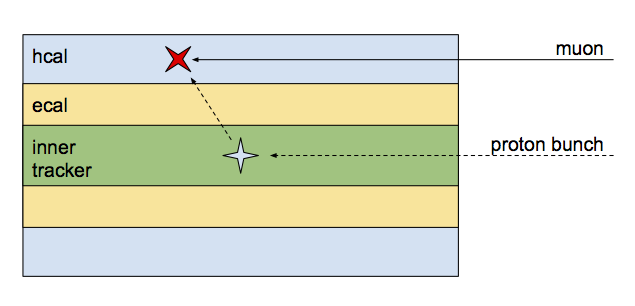
\includegraphics[width=\textwidth]{figures/beamHaloSketch.png}
  \caption{A sketch illustrating the timing differences between beam halo and particles from collisions.}
  \label{fig:beamHaloSketch}
  % sketched by Sascha in https://goo.gl/fw95iR
\end{figure}

Beam halo is most relevant for searches for displaced signatures without tracks in the inner tracker and for searches for decays in non-collision bunches (stopped particles)~\cite{Khachatryan:2015jha, Chatrchyan:2012dxa, Khachatryan:2010uf}. 

The contribution from beam halo can often be reduced by requiring high-momentum or high-energy reconstructed objects. One can also decrease the number of beam halo events by requiring central objects or vetoing forward muon system activity, since beam halo is usually in the very forward direction~\cite{Khachatryan:2015jha, Chatrchyan:2012dxa, Khachatryan:2010uf}. For inner tracker-based signatures, events from beam halo are rejected by requiring a minimum number of early hits.

Beam halo background can be estimated by using data control regions near $\phi=0$ and $\pi$. One could also identify cells with a low number or zero tracks that are assigned an early time. %where are the cells - calo? Do we have an example banana plot to show?

% -----------------------------------------------------------------------------------
\subsection{Cavern radiation} % Juliette
% -----------------------------------------------------------------------------------

There could also be radiation from the cavern walls, which might be a significant background in a LLP search. %more details about what this looks like in the detector are needed
Cavern radiation is usually not modelled in MC simulation.

Cavern radiation is most relevant for searches looking in non-collision data, that is, stopped-particle searches, and for searches using muon system information to form tracks and vertices. 

Cavern radiation can be estimated from data by collecting events triggered by random triggers when there are no collisions. It can also be estimated by overlaying a cavern radiation simulation with minimum-bias events from data.


% -----------------------------------------------------------------------------------
\section{Fake particle signatures} % Juliette
% -----------------------------------------------------------------------------------

Another type of background for LLP searches is that from signatures that mimic real particles in the detector, but are in fact fake. By this, we mean the contribution from spurious detector noise. Noise appears differently depending on the detector, but in general, it is characterized by a single and concentrated energy deposit or hit that does not correspond in time or space to any other energy deposits or hits in the detector. Noise is usually difficult to model with MC simulation.
%SM - general question: do we wanna use personal terms like "we do ..." or avoid it?
%JA - Yeah, maybe not, but I think this is a style question that would be good to have consistent across all sections of the white paper, so I suggest we leave it for when the sections get combined again.

Calorimeter detector noise is most relevant for searches looking in non-collision bunches and low-energy collisions~\cite{Khachatryan:2015jha, Chatrchyan:2012dxa, Khachatryan:2010uf}. Muon system noise is most relevant for searches that are also highly affected by cosmic-ray muons. 

Calorimeter noise can be rejected by vetoing single and concentrated energy deposits~\cite{Khachatryan:2015jha, Chatrchyan:2012dxa, Khachatryan:2010uf}. Muon system noise can be rejected by requiring high-quality muon tracks. 

Noise in both the calorimeters and the muon systems could be estimated by looking at dedicated cosmic data-taking runs and then applying some selection criteria to reject cosmic-ray muons. The remaining events would most likely be noise. 

% -----------------------------------------------------------------------------------
\section{Algorithmically induced fakes} % Sascha
% -----------------------------------------------------------------------------------

For searches that aim to reconstruct the decay vertex of a long-lived particle, and especially for long-lived particles decaying in the proximity of the interaction region, algorithmically induced fakes and/or instrumental backgrounds can be of importance. 

% -----------------------------------------------------------------------------------
\subsection{Random/merged vertices} % Sascha
% -----------------------------------------------------------------------------------

This type of background, illustrated in Figure~\ref{fig:mergedvertices} is especially important in the high-track-density environment close to the interaction region and arises from two main sources: two or more individual tracks crossing each other and getting reconstructed as a displaced vertex as well as two close-by low-mass vertices reconstructed as one high-mass displaced vertex (such a final merging/cleaning step is often part of vertexing algorithms to reduce fakes in standard vertexing).

\begin{figure}[h]
  \centering
  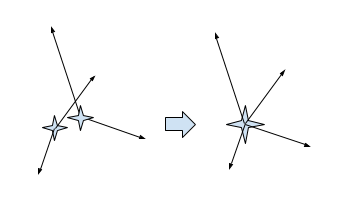
\includegraphics[width=0.7\textwidth]{figures/mergedvertices.png}
  \caption{Illustration of two close-by low-mass vertices being reconstructed as one high-mass vertex.}
  \label{fig:mergedvertices}
  % sketched by Sascha in https://goo.gl/fw95iR
\end{figure}

The former source is mostly suppressed by requirements originally targeting the removal of meta-stable SM particles: a minimum $|d_0|$ for tracks and a minimum distance between primary and a given displaced vertex. 

The latter source is obviously harder to suppress, though can be estimated by randomly merging vertices from distinct events. By studying number of reconstructed 'merged' high-mass vertices as a function of distance between the two low-multiplicity low-mass vertices that got 'merged' both with vertices from the same event as well as from different events and scaling them accordingly, an estimate for this background can be derived. This method has been successfully used the a recent ATLAS analysis searching for displaced vertices~\cite{Aaboud:2017iio}.

% -----------------------------------------------------------------------------------
\subsection{Randomly crossing tracks} % Sascha
% -----------------------------------------------------------------------------------

Typically of more relevance than merged vertices is the background stemming from low-mass vertices crossed by unrelated tracks, resulting in the reconstruction of a high-mass vertex, as illustrated in Figure~\ref{fig:randomcrossing}. The mass of the reconstructed displaced vertex is especially increased when the random track crosses the vertex in a direction that is perpendicular to the distance vector pointing from the primary vertex to the displaced one.

\begin{figure}[h]
  \centering
  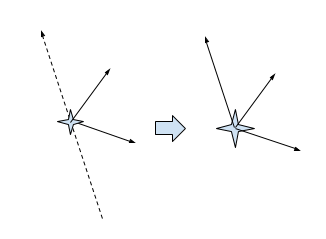
\includegraphics[width=0.7\textwidth]{figures/randomcrossing.png}
  \caption{Illustration of a low-mass vertex crossed by an unrelated track and being reconstructed as a high-mass vertex instead.}
  \label{fig:randomcrossing}
  % sketched by Sascha in https://goo.gl/fw95iR
\end{figure}

As demonstrated in detail in Ref.~\cite{Aaboud:2017iio}, this background can be estimated by constructing vertices (n-track) from lower-multiplicity ones (n--1-track) by adding pseudo-tracks, drawn randomly from data-driven track templates derived for various radial detector regions. The normalisation of the prediction is performed by comparing the n--1-track-based constructed vertices with the actual n-track vertices in all radial detector regions.

% -----------------------------------------------------------------------------------
\section{Summary} % all
% -----------------------------------------------------------------------------------

% We recommend that analyses provide separate background estimates for each source of background considered, rather than providing an estimate for one or more groups of different background sources.
